\documentclass[10pt]{article}
\usepackage{graphicx}

%%% Standard
\usepackage[margin=1in]{geometry} % One inch margins
\frenchspacing % No double spaces after periods.  Like this.
\usepackage{fancyhdr} % Easy to manage headers and footers
\pagestyle{fancyplain} % Formatting things
\linespread{1} % Single spaced
\setlength{\parindent}{0cm} % Don't indent new paragraphs
\newcommand{\psl}{6pt} % For consistency (\psl used again below)
\parskip \psl % Place a space between paragraphs instead
\usepackage{comment} % Adds \comment{} environment
\usepackage{lastpage} % For referencing last page
\usepackage{enumitem} % Include for \setlist{}
\setlist{nolistsep} % More compact spacing between environments
\setlist[itemize]{leftmargin=*} % Nice margins for itemize
\setlist[enumerate]{leftmargin=*} % and enumerate environments

%%% Standard math:
\usepackage{amsfonts,amssymb,amsmath,amsthm} % Math packages
\renewcommand{\t}{\text} % For text in math environment
\renewcommand{\c}{\cdot} % Multiplication dot in math
\newcommand{\f}[2]{\dfrac{#1}{#2}} % Shortcut for fractions
\newcommand{\p}[1]{\left(#1\right)} % Parenthesis
\renewcommand{\sp}[1]{\left[#1\right]} % Square parenthesis
\newcommand{\abs}[1]{\left|#1\right|} % Absolute value

%%% Physics symbols, vectors
\let\vepsilon\epsilon
\let\vphi\phi
\renewcommand{\epsilon}{\varepsilon} % Prettier epsilon
\renewcommand{\phi}{\varphi} % Prettier phi
\renewcommand{\l}{\ell} % Prettier l
\renewcommand{\v}[1]{\boldsymbol{\mathrm{#1}}} % Bold vectors
\newcommand{\uv}[1]{\hat{\boldsymbol{\mathrm{#1}}}} % Unit vectors
\newcommand{\del}{\v\nabla} % Del operator
\renewcommand{\d}{\partial} % Partial d
\newcommand{\fd}[2]{\f{d #1}{d #2}} % Derivative
\newcommand{\sd}[2]{\f{d^2 #1}{d^2 #2}} % Derivative
\newcommand{\fpd}[2]{\f{\d #1}{\d #2}} % Partial derivative
\newcommand{\spd}[2]{\f{\d^2 #1}{\d^2 #2}} % Partial derivative
\newcommand{\cx}[1]{\widetilde{#1}}

%%% Sections:
\usepackage{sectsty,titlesec} % Section options
\sectionfont{\large} % Section size

\renewcommand{\headrulewidth}{0pt} % Horizontal line in header
\cfoot{\thepage~of \pageref{LastPage}} % "X of Y" page labeling

\begin{document}

\section*{Generation}
\subsection*{Multilayer Spherical Phase Plates}
Using an electron beam, manufacturers are able to deposit SiO$_2$ into multilevel steps onto a substrate (Fig. \ref{mspp}). As the beam passes through this setup, the varying thickness causes the phase shift to differ based on the azimuthal angle. This causes the beam to develop a helical phase front, and consequently  form an optical vortex. In an ideal situation, the thickness of the phase plate would continuously increase rather than discrete intervals which would allow for a perfectly helical phase front, but the constraints of the manufacturing process do not allow for this. This method does not produce a pure Laguerre-Gaussian mode, but does effectively produce a prominent primary mode. \ref{MSPP}
\\\\

\begin{figure}
\centering
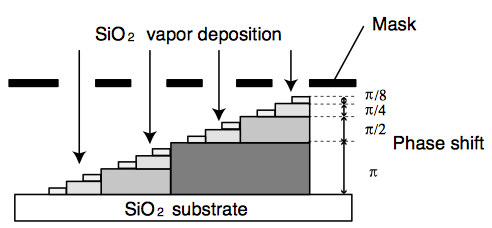
\includegraphics[scale=.5]{MSPP.jpg}
\caption{}
\label{mspp}
\end{figure}
New Line

\subsection*{Computer Generated Holography}
In CGH, an amplitude beam to be used as an optical vortex is directed through a hologram formed digitally and printed with extremely high resolution. The process for this formation is to incorporate both a planar wave used for reference, and the desired hologram obtained from an object wave. As these waves are combined, they for an interference pattern that can be printed and used as a filament for the optical vortex. When the beam propagates through this filament, there are an infinite number of diffraction orders produced with the first order beam containing the optical vortex. \ref{CGH}
\\\\\begin{center}
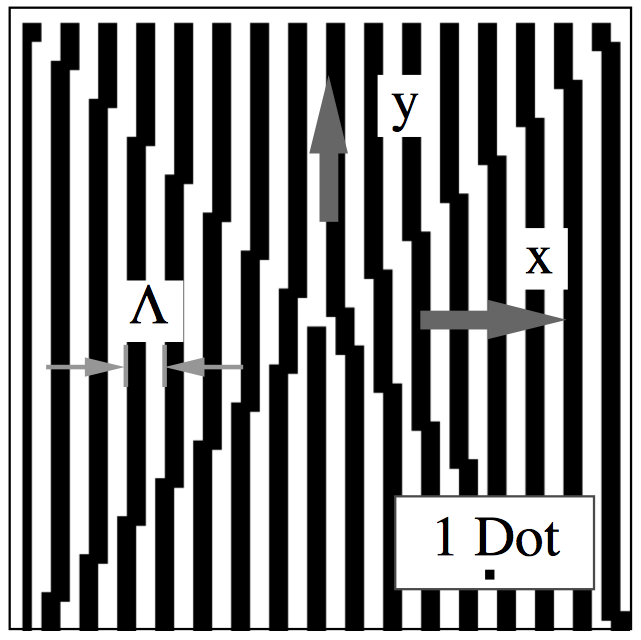
\includegraphics[scale=.3]{CGH.jpg}
\end{center}





\titlespacing{\section}{0pt}{\psl}{0pt}
\section*{Helical Modes of Light (Optical Vortices)}


The vector potential for a helical light beam traveling in the $\uv z$
and polarized in the $\uv x$ directions takes the form:
\begin{align*}
  \v A\p{r,\phi,z}&=A_0\f{w_0}{w}\sp{\f{r\sqrt 2}{w}}^\ell
  L^{\p{\ell}}_p\sp{2\f{r^2}{w^2}}\exp\sp{-\f{r^2}{w^2}}
  \exp\sp{-i\f{kr^2z}{2\p{z^2+z_R^2}}} \\
  &~~~~\times\exp\sp{i\p{2p+\ell+1}\arctan\p{\f z{z_R}}}
  \exp\p{i\ell\phi}\exp\p{-i\omega t} \uv x
\end{align*}
Here $A_0$ is a scaling factor, $w_0$ is the minimum beam waist, $w$
is the beam waist at the position $z$, $L^{\p{\ell}}_p$ is a
generalized Laguerre polynomial, $k$ is the wave vector, $\omega$ is
the frequency, $z_R$ is the Rayleigh length, $\ell$ is the topological
charge, and $p$ is the radial index. Parameters are given as follows:
\begin{align*}
  w=w_0\sqrt{1+z^2/z_R^2}
\end{align*}
\begin{align*}
  L^{\p{\ell}}_p\p{x}
  =\sum_{m=0}^p\p{-1}^m\f{\p{p+\ell}!}{\p{p-m}!\p{\ell+m}!m!}x^m
\end{align*}
\begin{align*}
  z_R=\f12 kw_0^2
\end{align*}
In particular, for $\p{\ell,p}=\p{3,1}$:
\begin{align*}
  L^{\p{3}}_1\p{x}=-x+4
\end{align*}
In the Coulomb gauge, we have $\del V=0$; for mutually perpendicular
$\v E$, $\v B$, and $\v k$ we must also have $\v k=k\uv z$. We can
then get the following electric ($\v E$) and magnetic ($\v B$) fields
from the complex component $\v A_I$ of the given vector potential:
\begin{align*}
  \v E=-\omega\v A_I=-\omega A_I\uv x &&& \v B=-\v k\times\v
  A_I=-kA_I\uv y
\end{align*}
The energy density $u$ is given by:
\begin{align*}
  u=\f12\p{\epsilon E^2+B^2/\mu} =\f12\p{\omega^2A_I^2+k^2A_I^2/\mu}
  =\f12\p{\epsilon\omega^2+\f{\omega^2}{c^2\mu}}A_I^2
  =\epsilon\omega^2A_I^2
\end{align*}
The Poynting vector $\v S$ is given by:
\begin{align*}
  \v S&=\v E\times\v B/\mu =-\omega\v A_I\times\p{-\v k\times\v
    A_I}/\mu =\f\omega\mu kA_I^2\uv k =\f{\omega^2}{c\mu}A_I^2\uv k
  =c\epsilon\omega^2A_I^2\uv k =cu\uv z
\end{align*}
Beam intensity $I$ is given by:
\begin{align*}
  I=\f{c\epsilon}2E^2=\f c2\epsilon\omega^2A_I^2=cu/2
\end{align*}
The Maxwell stress tensor $\sigma_{ij}$ in our case is given by:
\begin{align*}
  \sigma_{ij}=\epsilon\p{E_iE_j-\f12\delta_{ij}E^2}
  +\f1\mu\p{B_iB_j-\f12\delta_{ij}B^2} =\delta_{ij}\f12\p{\epsilon
    E^2+B^2/\mu}=\delta_{ij}u
\end{align*}
The force per unit volume $\v f=f_i\uv e_i$ on matter is in turn:
\begin{align*}
  f_i=\d_k\sigma_{ik}-\d_tS_i/c^2=\d_iu-\delta_{iz}\d_tu/c
\end{align*}

\end{document}